% This is samplepaper.tex, a sample chapter demonstrating the
% LLNCS macro package for Springer Computer Science proceedings;
% Version 2.20 of 2017/10/04
%
\documentclass[runningheads]{llncs}
%
\usepackage{graphicx}
% Used for displaying a sample figure. If possible, figure files should
% be included in EPS format.
%
% If you use the hyperref package, please uncomment the following line
% to display URLs in blue roman font according to Springer's eBook style:
% \renewcommand\UrlFont{\color{blue}\rmfamily}

\begin{document}
%
\title{Untrusted B2B Collaboration using the Blockchain}
%
%
\author{Jonas Beyer \and
Philipp Otto\and
S\"oren Tietb\"ohl}
%
\authorrunning{J. Beyer et al.}
% First names are abbreviated in the running head.
% If there are more than two authors, 'et al.' is used.
%
\institute{
Hasso-Plattner-Institut, Potsdam, Germany\\
\email{\{jonas.beyer,philipp.otto2,soeren.tietboehl\}@student.hpi.de}}
%
\maketitle % typeset the header of the contribution
%
\begin{abstract}
Lack of trust between communication partners is one of the major issues companies face when implementing business processes in a cross-organizational setting.
Blockchain is an emerging technology that enables decentralization and distribution of state without the need for a trusted central instance.
This allows for consensus in communication between otherwise untrusting parties.
In this paper we introduce Armadillo, an open-source prototype implementation for realizing business process choreographies using the Ethereum blockchain.
We present a user interface for connecting business processes with blockchain calls, as well as an underlying smart contract structure for inter-process communication.

\keywords{Blockchain \and Business Processes \and Ethereum \and Choreography \and Smart Contract \and BPMN}
\end{abstract}
%
%
%
\section{Introduction}

% Establish common ground with reader Worth readers time? Give some results

% Write it once at the start, then rewrite at the end
% use it to guide paper

% Important -> this structure will be expected

% Context (Topic / Terminology)
% Problem & Relevance (Problem - Costs / Current state - Gain)
% Related Work (Existing solutions / Shortcomings)
% Goals / Claims (Contribution, Sketch Results)
% Paper structure (The remainder of this paper is structured as follows ...)

% What is BPMN?
The Business Process Model Notation (BPMN) enables detailed documentation of business processes. This is used to realize complex inter-business processes which involve vast communication structures. One common problem is that within these processes the parties have to trust each other.
% What is Blockchain?

With the increasing spread of Blockchain technology, this problem could be rectified.
A Blockchain is a decentralized information-storage network. Information is stored in blocks, which are chained together via cryptograhic means. This means, that many participants can agree on a common public state of information without trusting each other. This technology is commonly used to realize virtual currencies, also called cryptocurrencies.
Ethereum is one implementation of the Blockchain concept, and it realizes a key feature called smart contracts.
Smart contracts are small programs, which are ran by the Blockchain network. They have very limited processing power, but they enable the execution of code which has a commonly known state. 

%What problems are there with BPMN that can be solved with Blockchain?
The problem of needing to trust each other when collaborating in a business process can be addressed by applying the benefits of blockchain technology. The Blockchain be used in several ways to facilitate trusted communication between untrusted parties.

% What approaches exist currently (Caterpillar \cite{lopez2017caterpillar}, Untrusted paper \cite{weber2016untrusted})
Current approaches aim to convert the functionality of traditional BPMN Engines to smart contracts on the Ethereum Blockchain.

Caterpillar~\cite{lopez2017caterpillar} features the implementation of most common BPMN elements. It enables the transformation of BPMN Models to smart contracts, which can be deployed and executed on the Blockchain.

Weber et al.~\cite{weber2016untrusted} realize Orchestrations on the Blockchain.

%What is our general Idea?
We want to expand on the work of Weber et al. and implement true choreographies. In their current approach they are using one central smart contract called a mediator / monitor which manages the Orchestration state.
We will have a set of smart contracts for every party, which will then communicate with each other to realize the choreography.
%What are our results? (briefly)

\section{Preliminary}
In the following section we present concepts and technologies that are related to our concept.

\subsection{Orchestrations and Choreographies}

\subsection{Blockchain}
A blockchain is a distributed ledger that allows users to find a concensus in decentralized applications.
It works by splitting information into blocks that are connected as a linked list. 
%TODO proof of work is only one possibility
%TODO explain more in depth?
Each block has to be signed in a way that is mathematically hard to calculate, but easy to verify.
Therefore users can verify if their local blockchain is valid.
If the same block is signed at the same time, a fork of the blockchain can happen, i.e. two versions of the same blockchain exist at the same time.
A concensus is reached by propagating the longest blockchain within the network until it is accepted by all parties of the network.

%TODO reference original blockchain paper
Blockchain technology is used in cryptocurrencies, most notably Bitcoin \cite{nakamoto2008bitcoin}.
The use in cryptocurrency has laid the foundation for a number of decentralized application besides financial ones.
Ethereum \cite{wood2014ethereum} is a cryptocurrency that also builds on blockchain technologies and allows users to execute code in the form of \emph{smart contracts}.
Smart contracts are Turing complete code artifacts, that can be deployed on the blockchain and have an interface that is callable by users. 
They can receive and send money, store information locally and emit events on the blockchain ledger.
When calling functions on a smart contract, users have to supply \emph{gas}, a unit that powers smart contract computations.
Contracts deplete gas for each operation and return excess gas back to the user.
This ensures that contracts are not running for an unlimited amount of time and that computations on the blockchain are expensive in order to avoid unnecessary operations being performed on-chain.

\section{Related Work}

summarize untrusted paper
summarize Caterpillar
acknowledge their Work
display the shortcomings

maybe also include Blockchain here? 

\section{Solution approach}

basic understanding/ intuition
-> make orchestration possible

use one contuous example

visualizations !!

\subsection{Contract Structure}

\subsection{Authorization}

\subsection{Decentralization}
% Decentralized contracts vs. central monitor
% Engine on chain vs. message channel

\section{Architecture}

\subsection{System overview}

\subsection{Per company setup}

\subsection{Interaction setup}

\subsection{Sending messages}

\begin{figure}
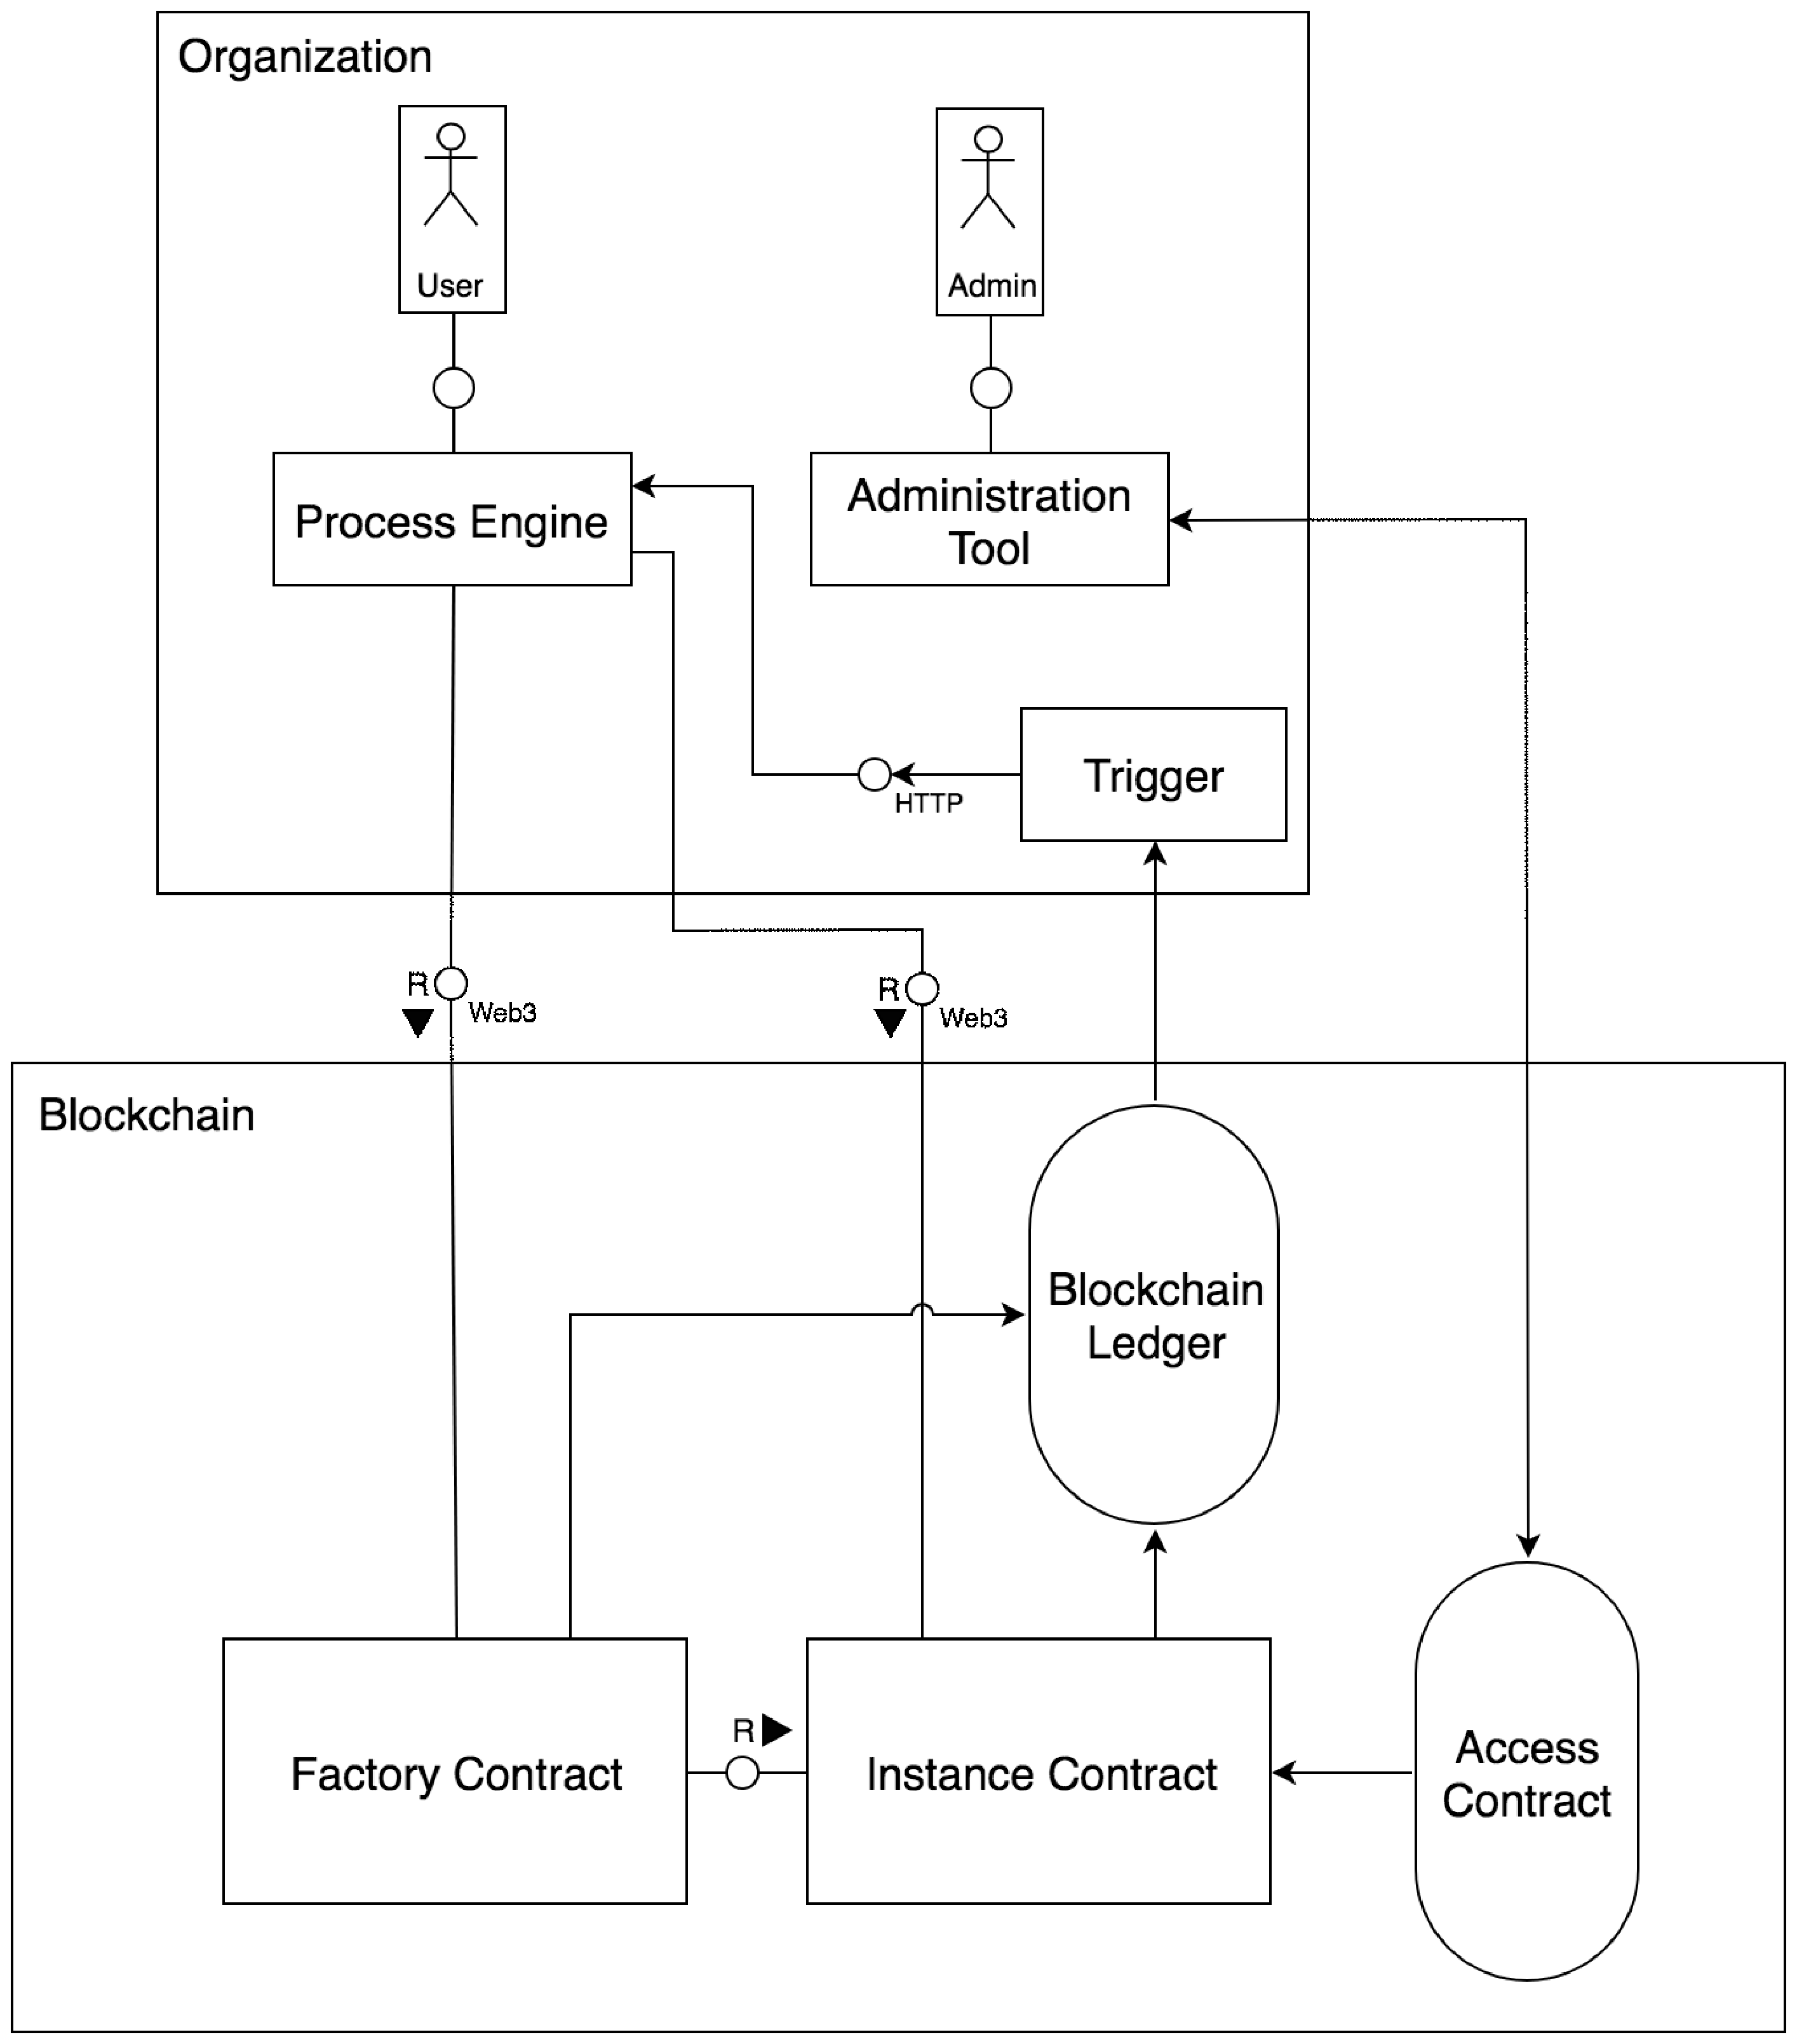
\includegraphics[width=\textwidth]{fig/system_diagram.eps}
\caption{The architecture of our design.} \label{fig1}
\end{figure}

\begin{figure}
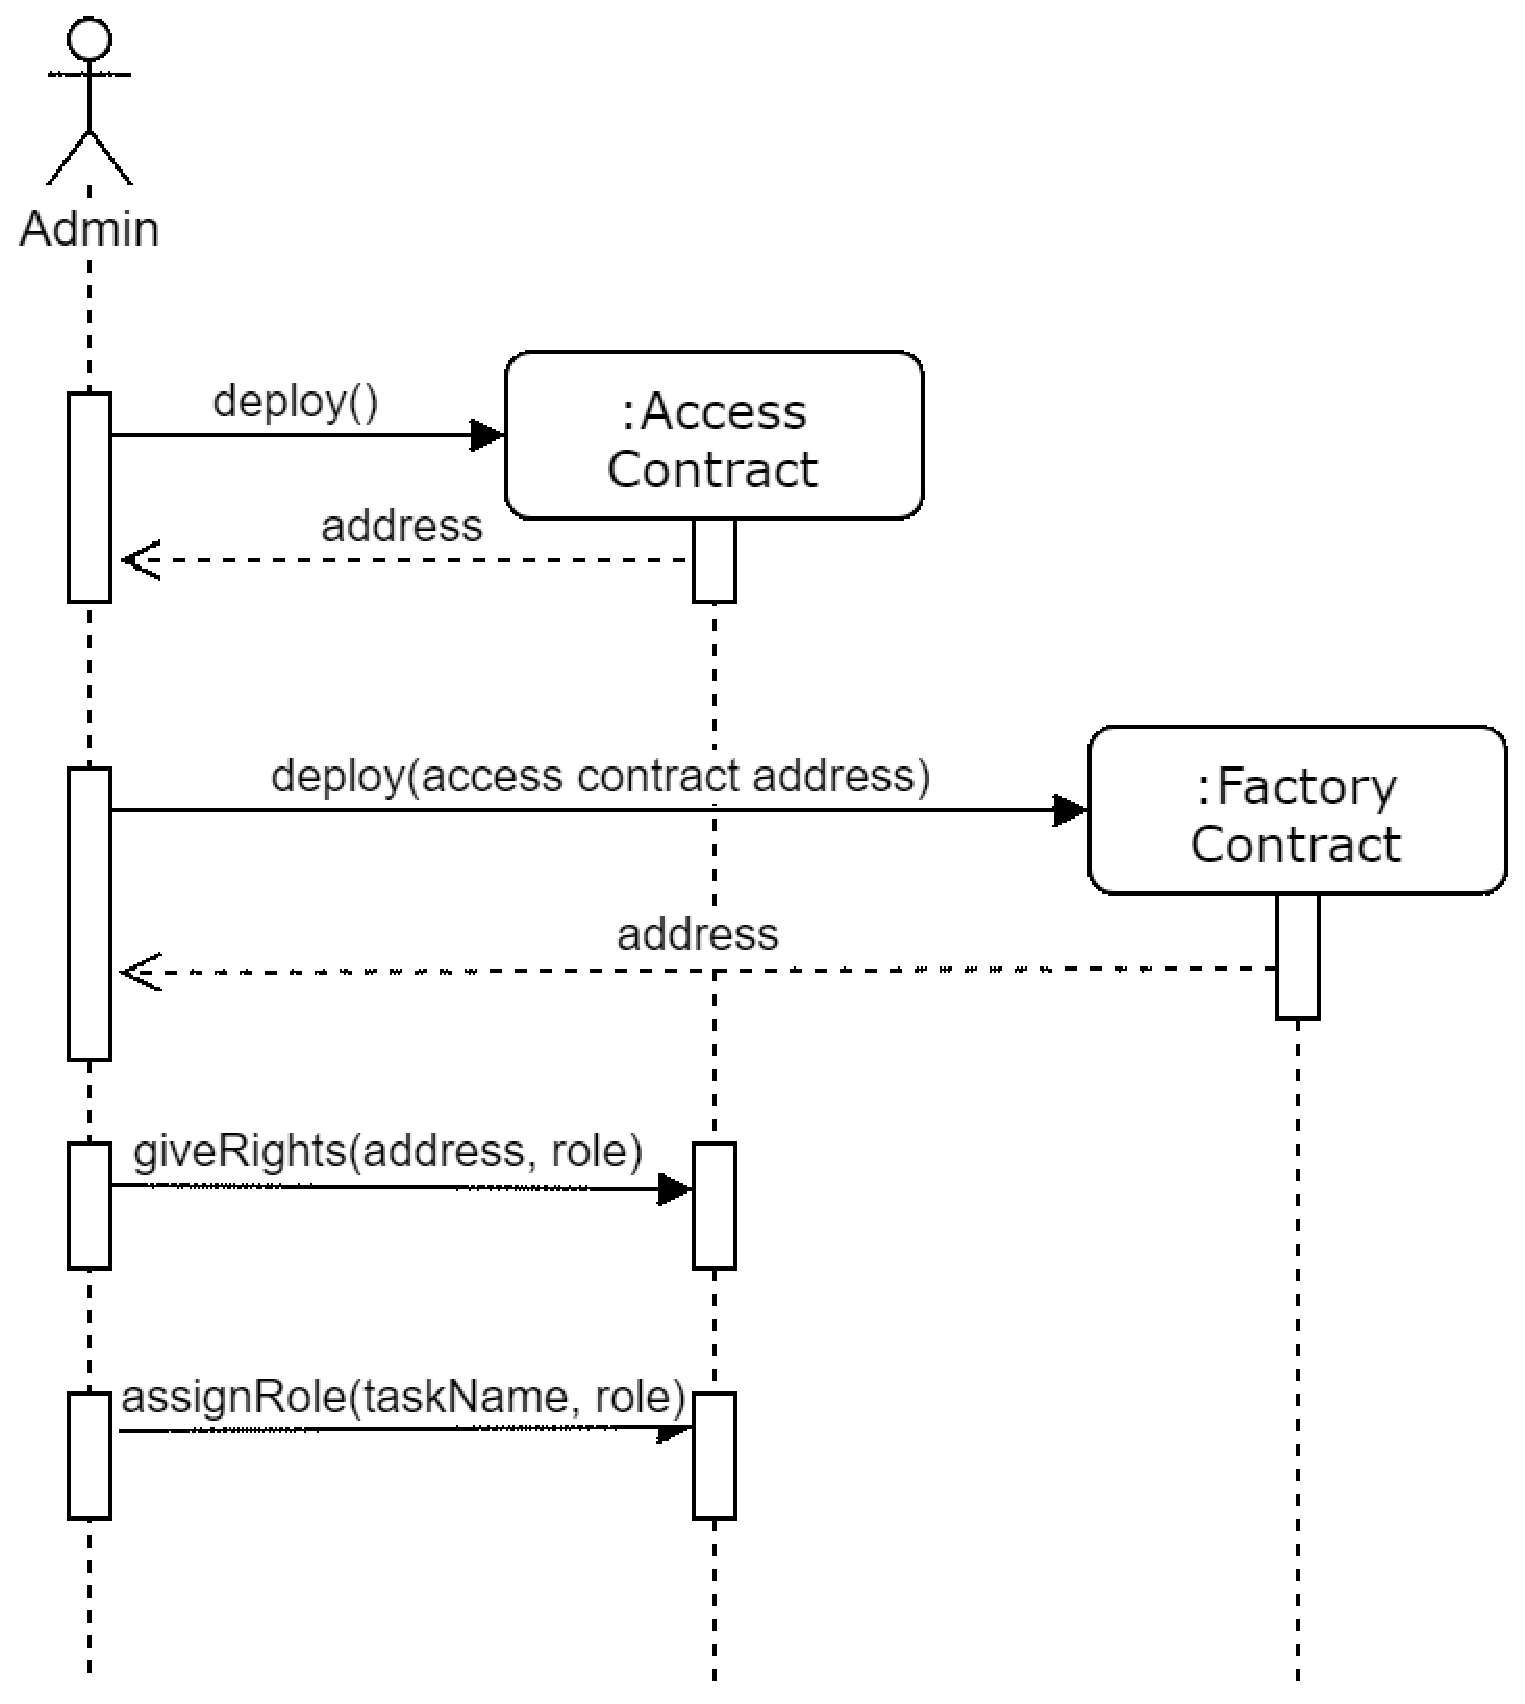
\includegraphics[width=\textwidth]{fig/initialization.eps}
\caption{An initialization process.} \label{fig2}
\end{figure}

\section{Implementation}

\subsection{Contracts}

\subsection{eth\_admin}

\subsection{armadillo}

\section{Evaluation}
%Gas cost
%Time for one instance
%Setup difficulty
%Security

%Mention problem of giving and removing right to change access rights
%But in the end one instance has to a be superadmin in the contract, if it is leaked there is a problem

\section{Conclusion}

%
% ---- Bibliography ----
%
% BibTeX users should specify bibliography style 'splncs04'.
% References will then be sorted and formatted in the correct style.
%
\bibliographystyle{splncs04}
\bibliography{references}

\end{document}
